%\documentclass{beamer}
\documentclass[handout]{beamer}

\geometry{margin=10pt,top=0pt}

\usepackage{multicol}
\usepackage{xcolor}
\usepackage{framed}
\usepackage{amsmath,amssymb,mathtools}
\usepackage{multirow}
\usepackage{graphicx}
\usepackage{subcaption}
\usepackage{tikz}

\usepackage[style=authoryear,
            bibstyle=authoryear,
            citestyle=numeric,
            hyperref=true,
            sorting=none]{biblatex}
\bibliography{../iep.bib}

\colorlet{TFFrameColor}{blue!50}
\colorlet{TFTitleColor}{white!75}

\setbeamertemplate{frametitle}{
  \hspace{-7pt}\insertframetitle
}

\graphicspath{{fig/}}

\title[IEP Investigation]{An Inverse Eigenvalue Problem (IEP) Investigation}
\author{Dan Folescu}
\date{}

\newif\ifafterftpause
\afterftpausetrue % default

\makeatletter
\def\beamer@checkframetitle{%
\@ifnextchar\bgroup\beamer@inlineframetitle{{}\ifafterftpause\pause\fi}}
\def\beamer@inlineframetitle#1{%
\@ifnextchar\bgroup{\frametitle{#1}\framesubtitle}{\frametitle{#1}\relax}%
\ifafterftpause\pause\fi
 }
\makeatother

\begin{document}
\beamertemplatenavigationsymbolsempty
{\afterftpausefalse \maketitle}

\section{Forward/Backward Eigenvalue Problems}

\begin{frame}{The Forward Problem}

  \begin{titled-frame}{Generalized Eigenvalue Problem}

    Given $A, B \in \mathbb{C}^{n \times n}$, find $(\lambda, \mathbf{x}) \in \mathbb{C} \times \left( \mathbb{C}^n - \{ \mathbf{0} \} \right)$ such that $$A \mathbf{x} = \lambda B \mathbf{x}.$$

  \end{titled-frame} \pause

  For $B = I$ this becomes the familiar linear eigenvalue problem (LEP). \pause

  Many algorithms exist to tackle this problem for general $A$~\cite{golubMatrixComputations2013}: \pause

  \begin{figure}
    \centering
    \begin{subfigure}{.3\textwidth}
      \includegraphics[width=\textwidth]{{powermethod}}
      \caption{Power Method}
      \label{subfig:powmeth}
    \end{subfigure} \pause
    \begin{subfigure}{.3\textwidth}
      \includegraphics[width=\textwidth]{{shiftandinvert}}
      \caption{Shift and Invert}
      \label{subfig:shiftinvert}
    \end{subfigure} \pause
    \begin{subfigure}{.3\textwidth}
      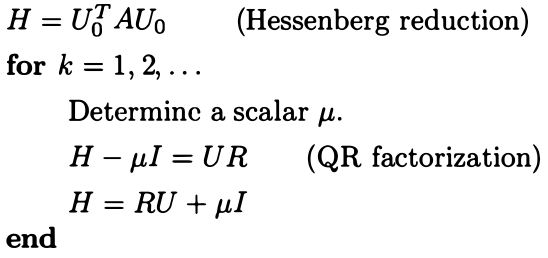
\includegraphics[width=\textwidth]{shiftedQR.png}
      \caption{QR Iteration}
      \label{subfig:QRiter}
    \end{subfigure}
  \end{figure}

\end{frame}

\begin{frame}{The Backwards Problem}

  Why?~\cite{chuInverseEigenvalueProblems2005} \pause

  \begin{itemize}
    \item system identification~\cite{coxOneCanHearSR2012} \pause
    \item principal component analysis~\cite{tenbergeRetrievingCorrelationMatrixP1999} \pause
    \item molecular spectroscopy~\cite{tomanMultiplicitySolutionsInverseJoMS1966} \pause
  \end{itemize}

  \begin{titled-frame}{Generalized IEP (GIEP)}

    Given $\lambda = \{ \lambda_1, \lambda_2, \cdots, \lambda_k \}$ for $k \leq n$, determine $A, B \in \mathbb{C}^{n \times n}$ so that $\det{(A - \lambda_i B)} = 0$ for $i = 1, 2, \cdots, k$.

  \end{titled-frame} \pause

  \begin{titled-frame}{A Novel GIEP Algorithm}

    Set $A = \text{diag}(\lambda_1, \lambda_2, \cdots, \lambda_k, 0, \cdots, 0)$ and $B = I$.

  \end{titled-frame} \pause

  \ldots Under-determined! We must impose constraints: \pause

  \begin{itemize}[<+->]
    \item spectral
    \item structural
  \end{itemize}

\end{frame}

\section{The Linear, Parameterized IEP (LiPIEP)}

\begin{frame}{A Structurally Constrained IEP (1)}

  Consider the following dynamical system:
  \begin{align*}
    \dot{\mathbf{x}}(t) &= A \mathbf{x}(t) + B \mathbf{u}(t)\\
    \mathbf{y}(t) &= C \mathbf{x}(t)
  \end{align*}
  where $A \in \mathbb{R}^{n \times n}, B \in \mathbb{R}^{n \times m}$, and $C \in \mathbb{R}^{p \times n}$.

  \pause

  \vspace{5pt}

  $\mathbf{u}(t) = K \mathbf{y}(t) = K C \mathbf{x}(t)$ induces the \emph{closed-loop} dynamical system:
  \begin{align*}
    \dot{ \mathbf{x} }(t) = ( A + B K C ) \mathbf{x}(t)
  \end{align*}

  \pause

  \begin{titled-frame}{Output Feedback Pole Assignment Problem (OfPAP)}

    Given $\lambda = \{ \lambda_i \}_{i = 1}^{n} \subseteq \mathbb{C}$ where $\overline{\lambda} = \lambda$ find $K \in \mathbb{R}^{m \times p}$ such that:
    \begin{align*}
      \sigma \left( A + B K C \right) = \{ \lambda_i \}_{i = 1}^{n}
    \end{align*}

  \end{titled-frame}

\end{frame}

\begin{frame}{A Structurally Constrained IEP (2)}

  \begin{titled-frame}{Linear Parameterized Inverse Eigenvalue Problem (LiPIEP)}

    For $\left\{ A_j \right\}_{j=1}^m \subset \mathcal{M} \subseteq \mathbb{C}^{n \times n}$, put $A( \mathbf{c} ) = A_0 + c_1 A_1 + \cdots + c_m A_m$.

    Given $\lambda = \{ \lambda_i \}_{i = 1}^{n} \subseteq \mathbb{C}$ where $\overline{\lambda} = \lambda$, find $\mathbf{c} = \begin{bmatrix} c_1 & \cdots & c_m \end{bmatrix}^T \in \mathbb{C}^{m}$ such that: $$ \sigma(A( \mathbf{c} )) \subseteq \{ \lambda_i \}_{i = 1}^{n} $$

  \end{titled-frame} \pause

  \textbf{Remark:} \pause

  \begin{itemize}
    \item When $m = 1, c_1 = 1, A_1 = B K C$ and $\subseteq \rightarrow =$, LiPIEP $\Leftrightarrow$ OfPAP. \pause
    \item When $\mathcal{M}$ is the set of symmetric, real, $n \times n$ matrices and $m = n$, we recover a variant of the LiPIEP, which we denote \emph{LiPIEP2}.
  \end{itemize}

\end{frame}

\begin{frame}{Simple Existence Results for the (Li)PIEP~\cite{chuInverseEigenvalueProblems2005}}

  \begin{titled-frame}{Theorem 1 (Xu, 1998)~\cite{hsuIntroductionInverseAlgebraic1998}}
    Given a set of $n$ complex numbers $\{ \lambda_k \}_{k = 1}^n$, then for almost all $\left\{ A_i \right\}_{i=0}^n \subset \mathbb{C}^{n \times n}$, there exists $\mathbf{c} \in \mathbb{C}^n$ such that $\sigma( A( \mathbf{c} )) = \{ \lambda_k \}_{k=1}^n$.
    Furthermore, there are at most $n!$ distinct solutions.
  \end{titled-frame} \pause

  \begin{titled-frame}{Theorem 2 (Helton et al., 1997)~\cite{heltonMatrixExtensionsEigenvalueTAMS1997}}
    For almost all $A_0 \in \mathbb{C}^{n \times n}$ and almost all $\{ \lambda_k \}_{k=1}^n$, there is a $\mathbf{c} \in \mathbb{C}^n$ such that $\sigma( A( \mathbf{c} ) ) = \{ \lambda_k \}_{k=1}^n$ \textbf{if and only if} the following two conditions hold:
    \begin{enumerate}
      \item The matrices $A_1, \cdots, A_n$ are linearly independent; and,
      \item $\text{trace}{\left( A_i \right)} \neq 0$ \emph{for some} $i = 1, 2, \cdots, n$.
    \end{enumerate}
  \end{titled-frame}

\end{frame}

\begin{frame}{Newton's Method for LiPIEP2}

  \textbf{Recall:} For differentiable $f \,:\, \mathbb{R} \rightarrow \mathbb{R}$, one Newton step is given as:
  \begin{align*}
  x^{(\nu + 1)} = x^{(\nu)} - ( f'( x^{(\nu)}) )^{-1} f( x^{(\nu)} ).
  \end{align*}

  \pause

  \textbf{Idea:} $f( x^{(\nu + 1)} )$ is a ``lift'' of the $x$-intercept of $f'( x^{(\nu)} )$. \pause

  \vspace{10pt}

  \begin{minipage}[h]{0.5\textwidth}
    Given $\lambda = \{ \lambda_k \}_{k=1}^n$, put
    \begin{align*}
      \mathcal{A} &\coloneqq \left\{ A( \mathbf{c} ) \,:\, \mathbf{c} \in \mathbb{R}^n \right\}\\
      \mathcal{M}(\Lambda) &\coloneqq \left\{ Q \Lambda Q^T \,:\, Q \in \mathcal{O}(n) \right\}\\
      &\text{where } \Lambda \coloneqq \text{diag}(\lambda).
    \end{align*}
  \end{minipage}%
  \hfill%
  \pause
  \begin{minipage}[h]{0.5\textwidth}
    \begin{figure}
      \captionsetup{justification=centering}
      \includegraphics[width=0.9\textwidth]{{LiPIEP2lift}}
      \caption*{Geometry of Newton's Method for PIEP~\cite{chuInverseEigenvalueProblems2005}}
      \label{fig:LiPIEP2lift}
    \end{figure}
  \end{minipage}

\end{frame}

{
  \afterftpausefalse

\begin{frame}
  \textbf{Code Aside}
\end{frame}

}

\section{The Stochastic IEP (StIEP)}

\begin{frame}{Definitions \& StIEP}

  Let $A = \left[ a_{ij} \right] \in \mathbb{R}^{n \times n}$.

  \vspace{10pt}

  We say $A$ is \emph{non-negative} if $a_{ij} \geq 0$ for $1 \leq i,j \leq n$. \pause

  \vspace{10pt}

  We say $A$ is \emph{(row) stochastic} if $\sum_{k=1}^n a_{ik} = 1$ for $i = 1, 2, \cdots, n$. \pause

  \begin{titled-frame}{StIEP}
    Given $\lambda = \{ \lambda_k \}_{k=1}^{n} \subseteq \mathbb{C}$ where $\overline{\lambda} = \lambda$, construct a (row) stochastic matrix $C \in \mathbb{R}^{n \times n}$ so that $$\sigma(C) = \{ \lambda_k \}_{k=1}^n $$
  \end{titled-frame}

\end{frame}

\begin{frame}{Restriction of the StIEP to Real Values}

  \begin{titled-frame}{Real Stochastic IEP (RStIEP)}

    \centering

    Given a set $\mathcal{S} = \{1\} \cup \{ \lambda_i \in \mathbb{R} \,:\, -1 \leq \lambda_i \leq 1 \}_{i = 2}^n,$ construct a stochastic matrix $C$ such that $\sigma(C) = \mathcal{S}$

  \end{titled-frame} \pause

  If $\lambda_1 = 1, \Lambda = \text{diag}{(\lambda_1, \cdots, \lambda_n)}$, then we may formulate the constrained optimization problem as:

  \begin{center}
    minimize\\$\left[ 2 \times \mathcal{J}(P,R) \right]^{1/2} \coloneqq \left\Vert P \Lambda P^{-1} - R \odot R \right\Vert = \left\Vert \Gamma(P) - \Xi(R) \right\Vert = \Vert \Delta(P,R) \Vert$\\subject to $P \in GL(\mathbb{R},n) $
  \end{center}
  where $\odot$ denotes the \emph{Hadamard} product.

  \pause

  With $[M, N] = MN - NM$ denoting the \emph{Lie bracket}, the gradient is given as~\autocite{chuInverseEigenvalueProblems2005}:
  \begin{align*}
    \nabla \mathcal{J}(P,R) = \left( \left[ \Delta(P,R), \Gamma(P)^T \right] P^{-T}, -2 \Delta(P,R) \odot R \right)
  \end{align*}

\end{frame}

{
  \afterftpausefalse

\begin{frame}

  \textbf{Code Aside} \pause

  \hspace{3cm}

  Now for the good part \ldots

\end{frame}

}

{
  \afterftpausefalse

\begin{frame}

  Let $\lambda \in \mathbb{R}, a \in \mathbb{R}^+ - \{0\}$ such that $\vert \lambda \vert < a$.

  \pause

  \vspace{5pt}

  Put $$ h_{\text{min}} = \lambda / (a + \lambda) \text{  and  } h_{\text{max}} = a / (a + \lambda),$$ and pick $r \in \mathbb{R}$ satisfying $\max{(h_{\text{min}},0)} \leq r \leq \min{(h_{\text{max}},1)}$.

  \pause

  \vspace{5pt}

  The \emph{scalar splitting operator}~\cite{ciampoliniDirectSolutionInverse2014} is defined to be $$\widehat{S}(a,\lambda,r) \coloneqq \frac{a}{h_{\text{max}}} \begin{pmatrix} r & h_{\text{max}} - r\\r - h_{\text{min}} & 1 - r \end{pmatrix}.$$

  \pause

  \textbf{Note:} Eigenvalues of $\widehat{S}(a,\lambda,r)$ are $a$ and $\lambda$.

  \pause

  Denote the \emph{state-splitting operator} by:
  \begin{align*}
    \arraycolsep=1.8pt\def\arraystretch{1.5}
    \widehat{S}_M(A,\lambda,r,k) \coloneqq \left( \begin{array}{c|c|c} \mathbf{A}_{11} & \underline{c}_{1k}^T & \mathbf{A}_{12}\\\hline \underline{r}_{k1} & a_{kk} & \underline{r}_{k2}\\\hline \mathbf{A}_{21} & \underline{c}_{2k}^T & \mathbf{A}_{22} \end{array} \right) \xrightarrow[k]{\text{split at}} \left( \begin{array}{c|c|c} \mathbf{A}_{11} & \begin{array}{cc} r\underline{c}_{1k}^T & (1-r) \underline{c}_{1k}^T \end{array} & \mathbf{A}_{12}\\\hline \underline{r}_{k1} & \multirow{2}{*}{$\widehat{S}(a_{kk},\lambda,r)$} & \underline{r}_{k2}\\\underline{r_{k1}} && \underline{r_{k2}}\\\hline \mathbf{A}_{21} & \begin{array}{cc} r \underline{c}_{2k}^T & (1-r) \underline{c}_{2k}^T \end{array} & \mathbf{A}_{22} \end{array} \right)
  \end{align*}

\end{frame}

}

\begin{frame}[t]{RStIEP Existence Results}

  \vspace{-15pt}

  \begin{titled-frame}{Theorem 3 (Sule\u{i}manova, 1949)~\cite{chuInverseEigenvalueProblems2005}}
    Any $n$ given real numbers $1, \lambda_2, \cdots, \lambda_n$ with $\vert \lambda_j \vert < 1$ are the spectrum of some $n \times n$ positive stochastic matrix if the sum of all $\vert \lambda_j \vert$ over those $\lambda_j < 0$ is less than $1$.
    If the $\lambda_j$'s are all negative the condition is also necessary.
  \end{titled-frame} \pause

  \begin{titled-frame}{Theorem 4 (Ciampolini, 2014)~\cite{ciampoliniDirectSolutionInverse2014}}
    If $\lambda = \{ \lambda_k \}_{k=1}^n$ has $0 \leq p \leq n$ positive values, then $\lambda$ is the spectrum of at least one stochastic matrix if:
    \begin{enumerate}
      \item $\max( \vert \lambda \vert ) = 1$; and,
      \item $\sum_{i=1}^n \lambda_i \geq 0$; and,
      \item the $(n-p)$ negative values of $\lambda$ can be grouped into $p$ clusters $\{ \mathcal{C}_\ell \}_{\ell=1}^{p}$ corresponding to a positive $\lambda_\ell$ such that $\left\vert \sum_{\gamma \in \mathcal{C}_\ell} \gamma \right\vert < \lambda_\ell$.
    \end{enumerate}
  \end{titled-frame} \pause

  \begin{tikzpicture}[remember picture, overlay]
    \node at (current page.center) {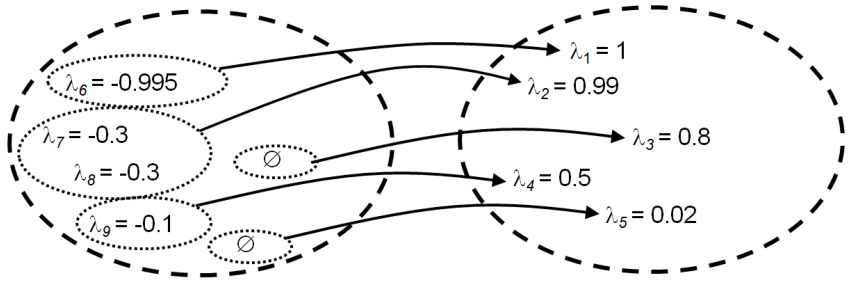
\includegraphics[width=0.9\textwidth]{neigclusters}};
  \end{tikzpicture}

\end{frame}

{
  \afterftpausefalse

\begin{frame}
  \textbf{Code Aside}
\end{frame}

}

{
  \afterftpausefalse

\begin{frame}
  \textbf{Questions?}
\end{frame}

}

\end{document}